\documentclass[aspectratio=169,10pt]{beamer}
\usepackage{fontspec}
\usepackage{polyglossia}\setdefaultlanguage{russian}
\setmainfont{DejaVu Serif}\setsansfont{DejaVu Sans}\setmonofont{DejaVu Sans Mono}
\usepackage{amsmath,booktabs}
\usetheme{Madrid}\usecolortheme{default}
\setbeamertemplate{navigation symbols}{}
\setbeamertemplate{footline}[frame number]
\setbeamerfont{frametitle}{size=\large}
\title{Исследование обобщённой дискретной модели}
\subtitle{Вариант 1, $k=4$}
\author{Власенко Ирина Владимировна}
\institute{ИММиКН, группа ПМИ-2.2, номер в списке $k=4$}
\date{28 октября 2026 г.}
\newcommand{\rc}{r_{\mathrm{crit}}}
\begin{document}
\begin{frame}\titlepage
\begin{center}\small Вариант 1:\quad $x_{n+1}=r\,x_n\Bigl(1-\dfrac{x_n+k x_n^2}{1+k}\Bigr)$,\quad $k=4$\end{center}
\end{frame}

\begin{frame}{Постановка задачи}
\begin{equation*}x_{n+1}=f(x_n)=r x_n\Bigl(1-\frac{x_n+4x_n^2}{5}\Bigr)=\frac r5\,(5x-x^2-4x^3)\end{equation*}
\begin{itemize}
\item $x_n$ --- нормированная плотность популяции в поколении $n$; $r>0$ --- скорость роста (воспроизводство при малой плотности: $f'(0)=r$).
\item Слагаемое $\frac{x+kx^2}{1+k}$ --- саморегуляция плотностью; $k$ задаёт её нелинейность. При $k=0$ --- классическое логистическое отображение $rx(1-x)$.
\item Нормировка: $f(1)=0$, а $\max f=f(c)\approx0{,}3569\,r$, $c=\frac{\sqrt{61}-1}{12}$. Поэтому отрезок $[0,1]$ инвариантен при $r\le r_{\max}\approx2{,}802$.
\item Цель: неподвижные точки, устойчивость, $\rc$, цикл периода 2, сценарий перехода к хаосу, сравнение с литературой.
\end{itemize}
\end{frame}

\begin{frame}{Литература и сравнение}
\small
\begin{enumerate}
\item R.\,M.\,May. \emph{Simple mathematical models with very complicated dynamics.} Nature 261 (1976), 459--467.
\item R.\,M.\,May, G.\,F.\,Oster. \emph{Bifurcations and dynamic complexity in simple ecological models.} Am.\ Nat.\ 110 (1976), 573--599.
\item A.\,G.\,Radwan. \emph{On some generalized discrete logistic maps.} J.\ Adv.\ Res.\ 4(2) (2013), 163--171.
\end{enumerate}
\textbf{Сравнение.}
\begin{itemize}
\item В [1,2] показано: простая нелинейная рекуррентная модель даёт каскад удвоений периода и хаос; в [3] обобщённые логистические отображения сводятся к классическому.
\item Общий случай: $f'(x^*)=-1\iff 4kx^2+3x-2(1+k)=0$. При $k=0$: $x^*=\frac23$, $\rc=3$ --- классическое значение для $rx(1-x)$. Для $k=4$: $\rc\approx2{,}151$, сдвиг в сторону меньших $r$ (согласуется качественно: сценарий тот же).
\item Отношения интервалов между бифуркациями: $4{,}57$ и $4{,}64$ --- к константе Фейгенбаума $\approx4{,}669$.
\end{itemize}
\end{frame}

\begin{frame}{Неподвижные точки и устойчивость}
$f(x)=x$: \quad $x^*_1=0$,\quad $4x^2+x+\frac5r-5=0\ \Rightarrow\ x^*_+=\dfrac{-1+\sqrt{81-80/r}}{8}$, $r>1$ (второй корень $<0$).
\begin{equation*}f'(x)=\tfrac r5(5-2x-12x^2),\qquad f'(0)=r\ \Rightarrow\ x^*_1\ \text{устойчива при }0<r<1.\end{equation*}
Для $x^*_+$ (используя $f(x^*)=x^*$): \quad $f'(x^*_+)=1-\dfrac{r\,x^*(1+8x^*)}{5}<1$, убывает с ростом $r$.
\begin{align*}f'(x^*_+)=-1\iff 16x^2+3x-10=0\ \Rightarrow\ x_{\rm crit}&=\tfrac{\sqrt{649}-3}{32}\approx0{,}70236,\\
\rc=\tfrac{5}{5-x_{\rm crit}-4x_{\rm crit}^2}&\approx\mathbf{2{,}1511}.\end{align*}
\textbf{Итог:} $x^*_+$ устойчива при $1<r<\rc$ (при $r=1$ --- транскритическая бифуркация, при $r=\rc$ --- удвоение периода).
\end{frame}

\begin{frame}{Цикл периода 2}
$f(f(x))-x=(f(x)-x)\,Q(x)$, $\deg Q=6$ (для кубического $f$ уравнение \textbf{не} квадратное). Симметрия: $s=x_1+x_2$, $p=x_1x_2$:
\begin{equation*}p=\tfrac{4s^2+s-5}{4}-\tfrac5{4r},\qquad 16r\,s^3+8r\,s^2-(19r+40)\,s-5(r+1)=0.\end{equation*}
Далее $x_{1,2}$ --- корни $t^2-st+p=0$; нужны $s^2-4p>0$ и $x_{1,2}\in(0,1)$.
\begin{itemize}
\item Существование: цикл рождается при $r=\rc$ (при $r=2{,}1501$ нет физичных корней, при $2{,}1521$ есть).
\item Устойчивость: $\mu=f'(x_1)f'(x_2)$, $|\mu|<1$. Из $\mu=-1$ (бисекция): $r_2\approx\mathbf{2{,}4136}$.
\item Цикл устойчив при $\rc<r<r_2$.
\end{itemize}
\end{frame}

\begin{frame}{Численно: сходимость и цикл}
\centering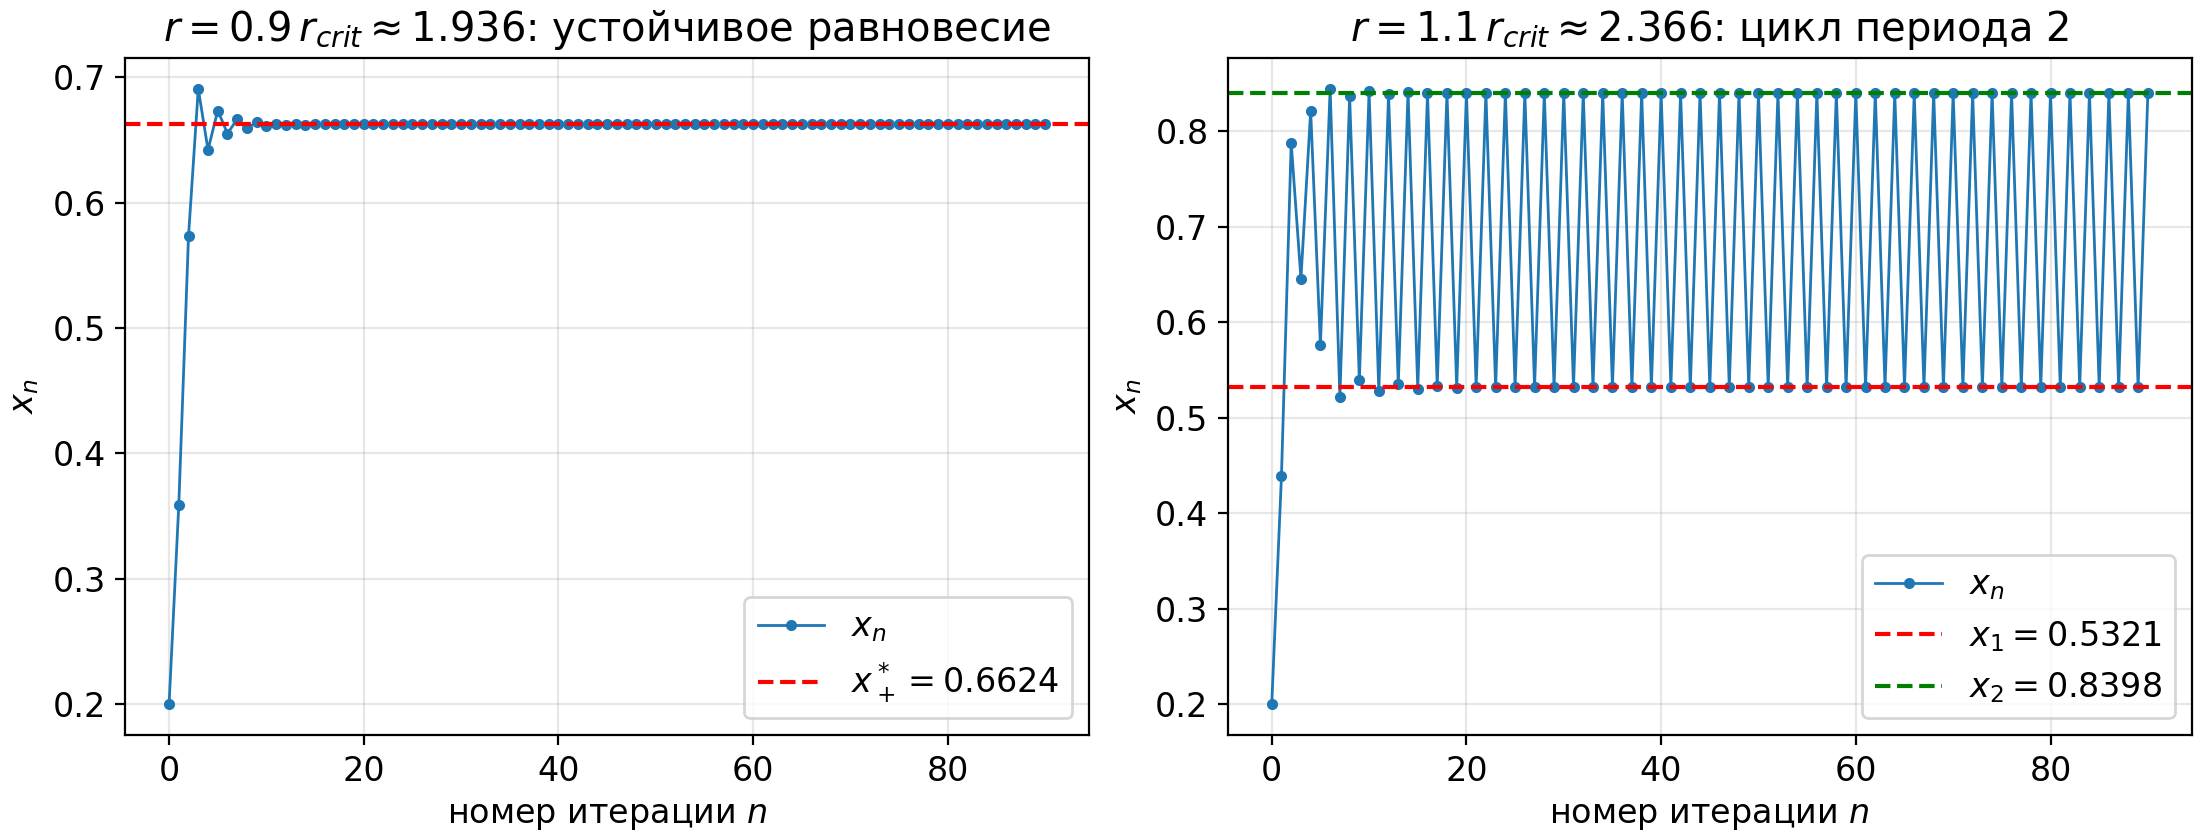
\includegraphics[width=.86\textwidth]{fig1.png}\\[-1mm]
\footnotesize\begin{tabular}{lcccc}\toprule
$r$ & $x_1$ & $x_2$ & $\varepsilon$ & $\mu$\\\midrule
$1{,}05\,\rc=2{,}2586$ & 0,58234 & 0,80527 & $8\cdot10^{-15}$ & $0{,}210$ (уст.)\\
$1{,}1\,\rc=2{,}3662$ & 0,53204 & 0,83987 & $3\cdot10^{-15}$ & $-0{,}621$ (уст.)\\
$1{,}2\,\rc=2{,}5813$ & 0,46388 & 0,88019 & $2\cdot10^{-15}$ & $-2{,}405$ (неуст.)\\\bottomrule\end{tabular}
\end{frame}

\begin{frame}{Бифуркации: диаграмма и ветви цикла}
\centering
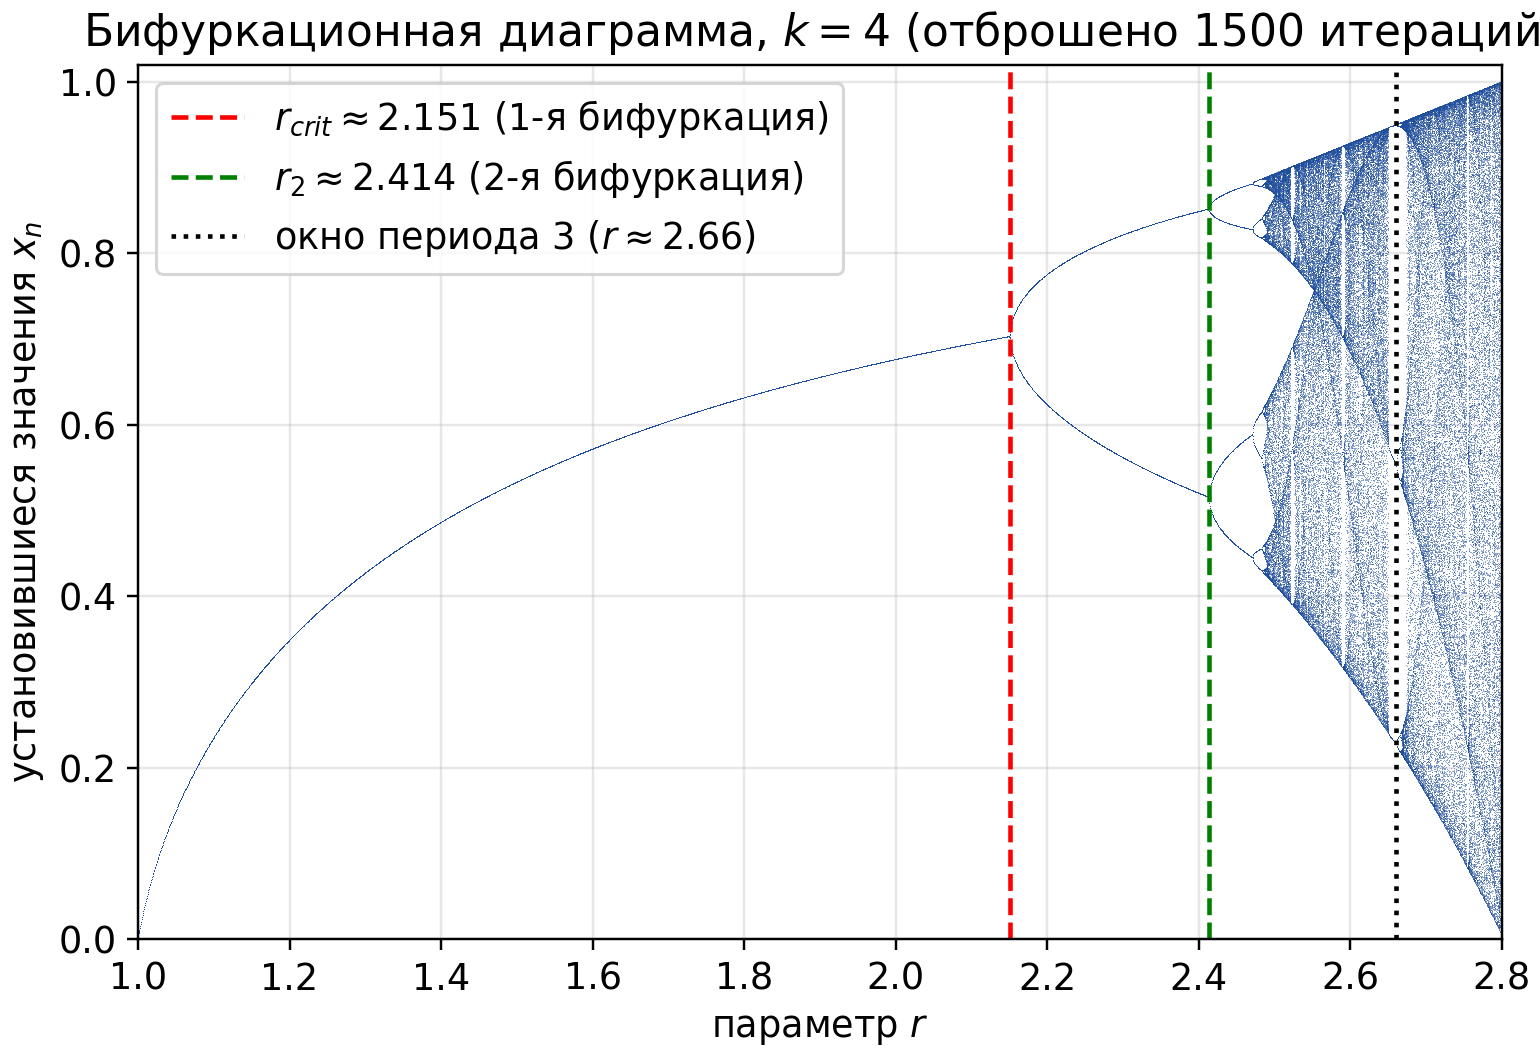
\includegraphics[width=.47\textwidth]{fig2.png}\hfill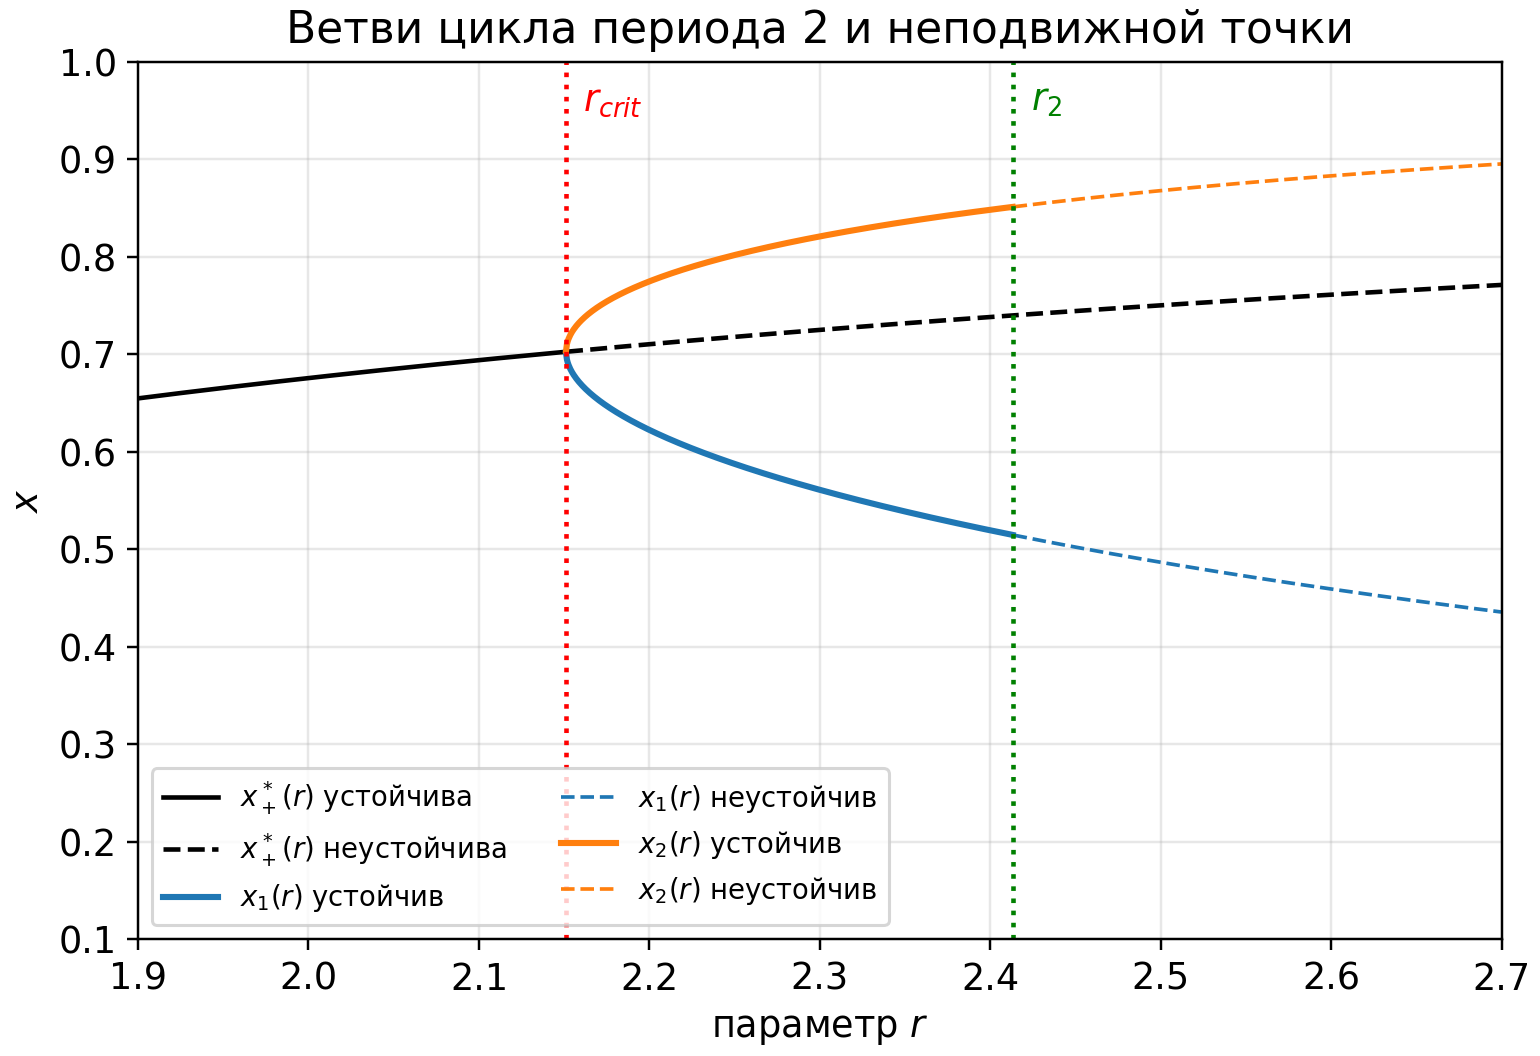
\includegraphics[width=.47\textwidth]{fig3.png}
\begin{itemize}\small
\item $\rc\approx2{,}1511$, $r_2\approx2{,}4136$, $r_3\approx2{,}4710$, $r_4\approx2{,}4834$: $\delta\approx4{,}57;\ 4{,}64$. Окно периода 3 при $r\approx2{,}66$.
\item Диаграмма заканчивается при $r_{\max}\approx2{,}802$ (дальше траектории уходят из $[0,1]$).
\end{itemize}
\end{frame}

\begin{frame}{Хаотический режим, $r=2{,}7$}
\centering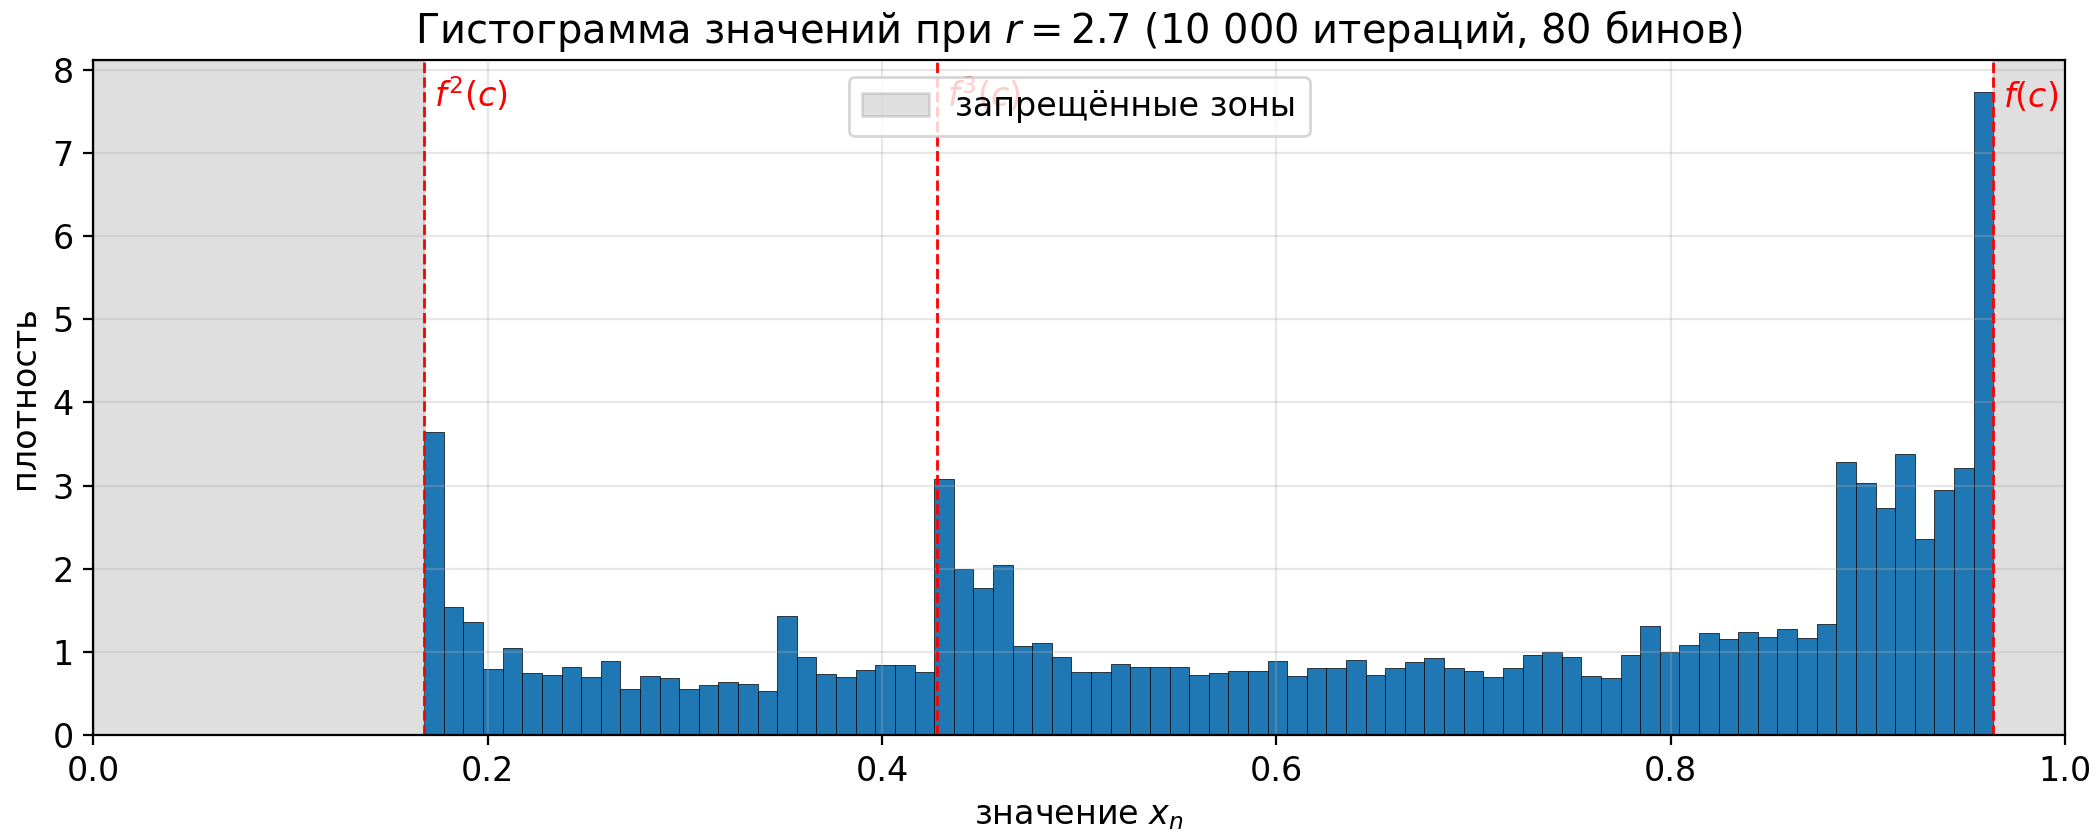
\includegraphics[width=.72\textwidth]{fig5.png}
\begin{itemize}\small
\item Показатель Ляпунова $\lambda\approx0{,}494>0$; близкие траектории ($10^{-10}$) расходятся за $\approx40$ итераций.
\item Запрещённые зоны: $x<f^2(c)\approx0{,}168$ и $x>f(c)\approx0{,}964$. Пики плотности у границ и в $f^3(c)\approx0{,}428$ --- образы критической точки; середина отрезка посещается реже.
\end{itemize}
\end{frame}

\begin{frame}{Выводы}
\begin{itemize}
\item Неподвижная точка $x^*_+=\frac{-1+\sqrt{81-80/r}}{8}$ устойчива при $1<r<\rc=2{,}1511$; $x^*_1=0$ --- при $0<r<1$.
\item Цикл периода 2 рождается при $\rc$ и устойчив при $\rc<r<r_2=2{,}4136$. Проверено: $\varepsilon\sim10^{-15}$, $|\mu|<1$.
\item Для кубического $f$ точки цикла находятся через кубическое уравнение для $s=x_1+x_2$ и квадратное для $x_{1,2}$ (не через одно квадратное).
\item Каскад удвоений ($r_3\approx2{,}4710$, $r_4\approx2{,}4834$, $\delta\approx4{,}6$) ведёт к хаосу; при $r=2{,}7$ $\lambda\approx0{,}494>0$, плотность ограничена зонами $[0{,}168;\,0{,}964]$.
\item Результаты качественно согласуются с [1--3]: при $k=0$ получаем классическое $\rc=3$.
\end{itemize}
\end{frame}

\begin{frame}{Использование ИИ}
\small\textbf{Ключевые промпты:}
\begin{enumerate}
\item Найти неподвижные точки модели при $k=4$ и показать преобразования.
\item Вывести $\rc$ из условия $f'(x^*)=-1$ и проверить подстановкой.
\item Написать код временных рядов, бифуркационной диаграммы и гистограммы.
\item Проверить, что численная пара удовлетворяет $f(x_1)=x_2$, $f(x_2)=x_1$.
\end{enumerate}
\textbf{Ошибки и исправления:}
\begin{itemize}
\item «Уравнение цикла квадратное»: для кубического $f$ степень $f\circ f-x$ делится на $f-x$ с остатком $\deg Q=6$; проверено в \texttt{sympy}, получено кубическое уравнение для $s$.
\item «Нерегулярный график = хаос»: недостаточно; посчитан $\lambda\approx0{,}494$ и чувствительность к $x_0$.
\end{itemize}
\textbf{Где ИИ помог:} выкладки, код. \textbf{Где нужна ручная проверка:} формулы, диапазоны $r$, выводы о хаосе.
\end{frame}
\end{document}
